\documentclass[a4paper,12pt]{article}

\usepackage{cmap}
\usepackage{amsmath}
\usepackage[T2A]{fontenc}
\usepackage[utf8]{inputenc}
\usepackage[english,russian]{babel}
\usepackage{graphicx}



\title{WGS, ECEF, ENU}
\author{}
\begin{document}
\maketitle

\section{Глобальные системы координат}
\quad

Декартова система координат ECEF начинается в центре масс земли,
ось $X$ направлена на Опорный мередиан,
ось $Z$ направлена на северный полюс,
ось $Y$ дополняет тройку до правой.

Эллипсоидальная система WGS на основе стандарта WGS84 основана на рефференсном эллипсоиде с параметрами
\begin{align} 
\label{eq:WGS_params}
&a = 6378137.0 \\
&f^{-1} = 298.257223563 \\
&b = a(1 - f) \\
&e = \sqrt{1 - b^2 / a^2}
\end{align}
с центром, совпадающем с центром системы ECEF,
нулевой меридиан -- Опорный меридиан,
нулевая параллель - экваториальная параллель.
Положение точки задается
широтой $\phi$,
долгоой $\lambda$,
высотой над эллипсоидом $h$.

\section{Переход от WGS к ECEF}
Переход от  WGS к ECEF:

\begin{align} 
\begin{split} \label{eq:WGS_to_ECEF}
&x = (\frac{a}{\chi} + h) \cos \phi \cos \lambda \\
&y = (\frac{a}{\chi} + h) \cos \phi \sin \lambda \\
&z = \Big(\frac{a(1-e^2)}{\chi} + h \Big) \sin \phi,
\end{split}
\end{align}
где
\begin{align*} 
\chi = \sqrt{1 - e^2 \sin^2 \phi}.
\end{align*}

\section{Переход от ECEF к WGS}

Обратное преобразование основано на численных методах
[Osen K. Accurate Conversion of Earth-Fixed Earth-Centered Coordinates to Geodetic Coordinates. – 2017.]
\begin{align} 
&w^2 = x^2 + y^2 \\
&l = e^2 / 2 \\
&m = w^2 / a^2 \\
&n = z^2(1-e^2) / a^2 \\
&p = (m + n - 4l^2) / 6 \\
&G = mnl^2 \\&m = w^2 / a^2 \\
&H = 2p^3 + G \\
&if \\
&C = \sqrt[3]{H + G + 2 \sqrt{HG}} / \sqrt[3]{2} \\
&i = -(2l^2 + m + n) / 2 \\
&P = p^2 \\
&\beta = i/3 - C - P/C \\
&k = l^2(l^2 - m - n) \\
&t = \sqrt{\sqrt{\beta^2-k} - (\beta + i)/2} - \text{sign} (m-n) \sqrt{|\beta - i| / 2} \\
\end{align}
\begin{align} 
&F = t^4 + 2it^2 + 2l(m-n)t + k \\
&dF / dt = 4t^3 + 4it + 2l (m-n) \\
&\Delta t = -F / (dF/dt) \\
&u = t + \Delta t + l\\
&v = t + \Delta t - l\\
&w = \sqrt{w^2} \\
&\phi = \text{atan2} (zu, wv) \\
&\Delta w = w(1-1/u) \\
&\Delta z = z(1-(1 - e^2)/v) \\
&h = \text{sign} (u -1) \sqrt {(\Delta w)^2 + (\Delta z)^2} \\
&\lambda = \text{atan2} (y, x)
\end{align}

\section{Локальная система ENU}

Введем ENU локальную систему координат,
начало которой лежит в точке $\omega_0 = (\phi_0, \lambda_0, h_0)$,
ось $X$ направлена на восток,
ось $Y$ на север,
ось $Z$ нормально поверхности эллипсоида и дополняет систему до правой тройки.

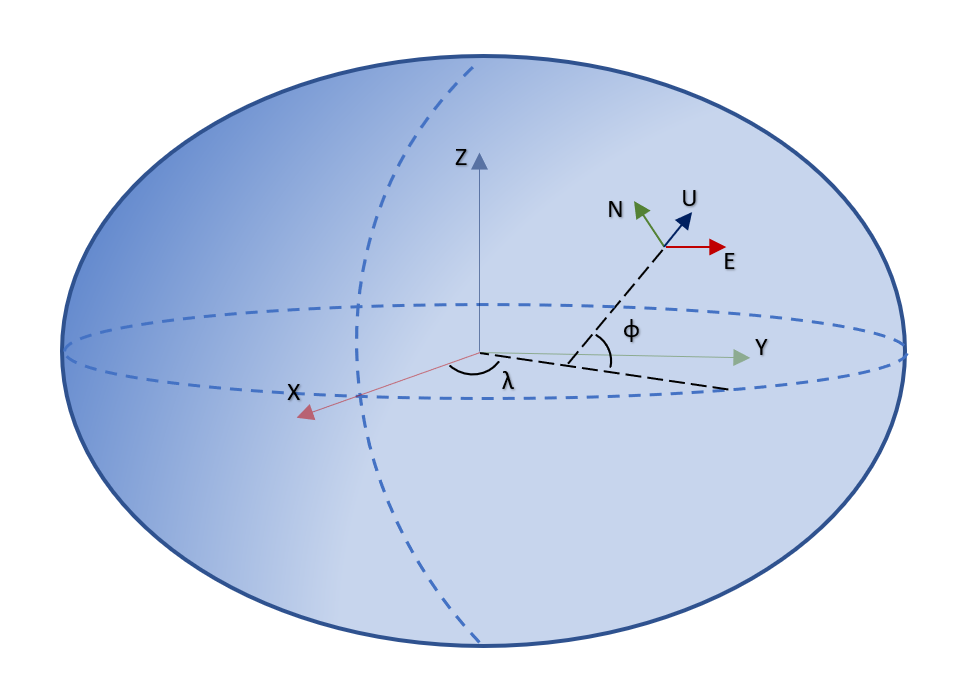
\includegraphics[width=\textwidth]{ecef_enu}

Для перехода из ECEF в ENU потребуется два последовательных поворота:
вокруг оси $Z$ на угол $\lambda$
и вокруг повернутой оси $Y'$ на угол $\phi$.
Тогда, матрица поворота
\begin{equation}
R_{ECEF}^{ENU} = 
\begin{bmatrix} \label{eq:R_ECEF_ENU}
&-\sin \lambda &\cos \lambda &0 \\
&-\sin \phi \cos \lambda &-\sin \phi \sin \lambda &\cos \phi \\
&\cos \phi \cos \lambda &\cos \phi \sin \lambda &\sin \phi 
\end{bmatrix}
.
\end{equation}


\section{Переход ECEF к ENU}
Чтобы найти координаты произвольной точки $\omega_1 = (\phi_1, \lambda_1, h_1)$ в ENU,
преобразуем $\omega_0$ и $\omega_1$ в ECEF согласно уравнениям \eqref{eq:WGS_to_ECEF}
и найдем  $r_0 = (x_0, y_0, z_0)$, $r_1 = (x_1, y_1, z_1)$.
Тогда, координаты точки $\omega_1$ могут быть записаны в ENU, как
\begin{align} 
\rho_1 = R_{ECEF}^{ENU} (r_1 - r_0).
\end{align}

\section{Переход ENU к ECEF}
Аналогично, для того, чтобы найти координаты точки в ECEF, зная их в ENU:
\begin{align} 
r_1 = r_0 + R_{ENU}^{ECEF} \rho_1.
\end{align}

\end{document}


